%; whizzy paragraph -pdf xpdf -latex ./whizzypdfptex.sh
%; whizzy-paragraph "^\\\\begin{frame}\\|\\\\emtext"
% latex beamer presentation.
% platex, latex-beamer でコンパイルすることを想定。 

%     Tokyo Debian Meeting resources
%     Copyright (C) 2012 Junichi Uekawa
%     Copyright (C) 2016 Nobuhiro Iwamatsu

%     This program is free software; you can redistribute it and/or modify
%     it under the terms of the GNU General Public License as published by
%     the Free Software Foundation; either version 2 of the License, or
%     (at your option) any later version.

%     This program is distributed in the hope that it will be useful,
%     but WITHOUT ANY WARRANTY; without even the implied warreanty of
%     MERCHANTABILITY or FITNESS FOR A PARTICULAR PURPOSE.  See the
%     GNU General Public License for more details.

%     You should have received a copy of the GNU General Public License
%     along with this program; if not, write to the Free Software
%     Foundation, Inc., 51 Franklin St, Fifth Floor, Boston, MA  02110-1301 USA

\documentclass[cjk,dvipdfmx,12pt]{beamer}
\usetheme{Tokyo}
\usepackage{monthlypresentation}

%  preview (shell-command (concat "evince " (replace-regexp-in-string "tex$" "pdf"(buffer-file-name)) "&")) 
%  presentation (shell-command (concat "xpdf -fullscreen " (replace-regexp-in-string "tex$" "pdf"(buffer-file-name)) "&"))
%  presentation (shell-command (concat "evince " (replace-regexp-in-string "tex$" "pdf"(buffer-file-name)) "&"))

%http://www.naney.org/diki/dk/hyperref.html
%日本語EUC系環境の時
\AtBeginDvi{\special{pdf:tounicode EUC-UCS2}}
%シフトJIS系環境の時
%\AtBeginDvi{\special{pdf:tounicode 90ms-RKSJ-UCS2}}

\newenvironment{commandlinesmall}%
{\VerbatimEnvironment
  \begin{Sbox}\begin{minipage}{1.0\hsize}\begin{fontsize}{8}{8} \begin{BVerbatim}}%
{\end{BVerbatim}\end{fontsize}\end{minipage}\end{Sbox}
  \setlength{\fboxsep}{8pt}
% start on a new paragraph

\vspace{6pt}% skip before
\fcolorbox{dancerdarkblue}{dancerlightblue}{\TheSbox}

\vspace{6pt}% skip after
}
%end of commandlinesmall

\title{東京エリアDebian勉強会\\Debian JP Project}
\subtitle{OSC 2019 Tokyo/Spring (第171回出張勉強会)}
\author{杉本 典充\\ dictoss@live.jp}
\date{2019年2月23日}
\logo{
\includegraphics[width=8cm]{image200607/openlogo-light.eps}}

\begin{document}

\section{表紙}

\begin{frame}
\titlepage{}
\end{frame}

\section{目次}

\begin{frame}{Agenda}
  \begin{itemize}
  \item Debian とは?
  \item Debian JP Project と Debian 勉強会
  \item Debian 10 (Buster)
  \item Debian Updates
  \item 今後のイベント
  \end{itemize}
\end{frame}

%-------------------

\section{Debian とは?}

\begin{frame}\begin{center}\Huge{Debian とは?}\end{center}\end{frame}


\begin{frame}{Debian とは?}

{\color{red}{フリー/オープン}}な{\color{red}{ユニバーサル}}オペレーティングシステム を作成しようとするボランティアベースのプロジェクト

\begin{table}[htb]
  \begin{tabular}{|c|c|c|}
    \hline
    ディストリ & 企業 & ボランティア \\ \hline
    Fedora & RedHat支援あり & あり  \\ \hline
    RHEL & RedHat & なし  \\ \hline
    CentOS & RedHat支援あり & あり \\ \hline
    \color{red}{Debian}  & \color{red}{なし} & \color{red}{あり} \\ \hline
    Ubuntu  & Canonical & あり \\ \hline
    openSUSE & SUSE支援あり & あり \\ \hline
    SLES & SUSE & なし \\ \hline
  \end{tabular}
\end{table}

\end{frame}

\begin{frame}{Debian とは?}
 世界規模で開発が行われており、63ヶ国、約1000名のDebian公式開発者が開発を行
 っている。パッケージメンテナや翻訳などの貢献者も入れるともっと多くの開発者が参加
 していることになる。
 \begin{center}
%%%   \includegraphics[width=0.7\hsize]{image201707/group_photo_t.jpg}
 \end{center}
\end{frame}


\begin{frame}{Debian とは?}

\begin{itemize}
  \item 様々な用途に使える汎用的な作り
    \begin{itemize}
    \item デスクトップPC、ノートPCなどの普段利用するコンピュータのOS
    \item Linuxサーバ (例:webサーバのシェア:\url{https://w3techs.com/technologies/details/os-linux/all/all})
    \item 組込デバイスのベースOS (多くのCPUで動作する)
  \end{itemize}
  \item 「Debian」ベースな派生OSの源流
  \begin{itemize}
    \item Ubuntu や Raspbian といったディストリビューションのベースはDebian
    \item 派生先のディストリビューションと相互に情報交換をして開発している
  \end{itemize}
\end{itemize}

\end{frame}


\begin{frame}{Debian とは?}

\begin{itemize}
  \item 2019年2月の時点で、最新版は {\color{red}{Debian 9.8}} (コードネーム: Stretch)
  \begin{itemize}
    \item パッケージ数は{\color{red}{約51000}}を提供
    \item 公式にサポートするCPUアーキテクチャは{\color{red}{10}}
  \end{itemize}
  \item {\color{red}{約2年毎}}にリリース
  \item 次のリリース Debian 10 (コードネーム: {\color{red}{}}Buster)は 2019年中頃にリリースすると思われる
  \item コードネームはトイ・ストーリーのキャラクターを採用
\end{itemize}

\end{frame}


\begin{frame}{Debian とは?}

\begin{itemize}
  \item Debian 社会契約
    \begin{itemize}
      \item Debian 開発者たちが目指すフリーソフトウェアコミュニティーの在り方
    \end{itemize}
  \item Debian フリーソフトウェアガイドライン(DFSG)
    \begin{itemize}
      \item Debian 社会契約の一部
      \item Debian が考えるフリーソフトウェアの定義
      \item オープンソースの定義のひな形にもなっている
    \end{itemize}
  \item Debian Policy
    \begin{itemize}
      \item \url{https://www.debian.org/doc/debian-policy/}
      \item Debian パッケージの区分、内容やルール、ファイル配置の方針を定義
    \end{itemize}
\end{itemize}

\end{frame}


\begin{frame}{Debian とは?}
まとめると
\begin{itemize}
  \item Debianはフリー/オープンなオペレーティングシステム (OS)を作成しようとするボランティアベースのプロジェクト
  \item 自分たちの考えるフリーという言葉に関する定義、開発目的、パッケージングポリシーを厳格に決めている
  \item 世界中に1000人以上の開発者がおり、他のディストリビューションのベースとして採用されている
  \item 約2年毎にリリースが行われ、多くのパッケージとアーキテクチャをサポートしている
  \item 上記のような特徴から様々なところで利用されているLinuxディストリビューション
\end{itemize}

\end{frame}

%------------------


\section{Debian JP Project と Debian勉強会}


\begin{frame}
  \begin{center}\Huge{Debian JP Project\\と\\Debian勉強会}\end{center}
\end{frame}

\subsection{Debian JP Projectとは}
  
\begin{frame}{Debian JP Project とは?}

\begin{itemize}
  \item 日本でDebianを普及させることを目的とした任意団体
  \item 活動内容
  \begin{itemize}
    \item Debian の日本語による情報発信
    \item ユーザとの情報交換
    \item Debian 開発者、パッケージメンテナの育成など
  \end{itemize}
\end{itemize}

\end{frame}

\subsection{Debian勉強会}

\begin{frame}
  
\frametitle{Debian勉強会}
\begin{itemize}
 \item 2005年1月開始
 \item Debian Developer 上川さん発起人
\item 東京と関西で月に一回コンスタントに開催しているDebian開発者、ユーザによる勉強会
\end{itemize}

\end{frame}


\begin{frame}

\frametitle{Debian勉強会:解決したい内容}
\begin{itemize}
 \item<1-> 問題
       \begin{itemize}
	\item MLとIRCで情報交換していた
	\item face-to-faceであう場所がない
	\item まとまったドキュメントが出てこない
       \end{itemize}
 \item<2-> Debian勉強会の提案
       \begin{itemize}
	\item 定期的に集まる
	\item 資料を作成する。(GPLで!) \\
	  {\small \url{https://salsa.debian.org/tokyodebian-team/monthly-report}}
       \end{itemize}
\end{itemize}

\end{frame}


\subsection{最近の勉強会}


\begin{frame}
  
\frametitle{Debian勉強会:最近の勉強会}
  
\begin{itemize}
  %\item Debian Weekly News Quiz
  \item Debian 界隈やパッケージング関連の話題など専門の人に話を聞く
  \item Debianで気になった事柄を調べてレポートする
  \item 前回の内容(東京 1月):
	\begin{itemize}
	\item 場所: サイオスさん
    \item Debian Bug Squash Party Tokyo 2019-01
    \item 次リリースのDebian 10 Busterのバグ潰し会を実施
	\end{itemize}
  \item 各地のイベントでDebian普及活動
	\begin{itemize}
      \item OSC2018北海道、OSC2018京都、OSC2018東京
      \item 関西オープンフォーラム
	  \item Debian/Ubuntu ユーザミートアップ in 札幌
	\end{itemize}
\end{itemize}

\end{frame}

%-----------------------

\section{次期安定版 Debian 10 (Buster)}

\begin{frame}
  \begin{center}\Huge{Debian 10 (Buster)}\end{center}
  %\begin{center}\Huge{Debian 10 (Buster)\\リリースおめでとう!}\end{center}
\end{frame}


\begin{frame}{Debian 10 Buster}% [containsverbatim]

Debian 10 (コードネーム:Buster)

\begin{itemize}
\item 現在開発を進めている次の安定版リリース
\item Debianはtime-based freezeを採用しており、およそ2年毎のリリースを目指す
\end{itemize}
  \begin{center}
    %\includegraphics[width=0.6\hsize]{image201902/buster.jpg}
    % https://pixar.fandom.com/wiki/Buster
  \end{center}
\end{frame}


\subsection{テーマ}


\begin{frame}{Debian 10 Buster}% [containsverbatim]

テーマはAlex Makasさん提案の「futurePrototype」に決定。
  
\begin{center}
  
\includegraphics[width=0.75\hsize]{image201902/futurePrototype-wallpaper-1920x1080.png}
\end{center}

\url{https://bits.debian.org/tag/artwork.html}

\url{https://wiki.debian.org/DebianArt/Themes/futurePrototype}

\end{frame}


\subsection{提供ソフトウェアのバージョン}


\begin{frame}{Debian 10 Buster}% [containsverbatim]

ソフトウェアは以下のバージョンでテスト中

\begin{itemize}
\item Linux カーネル 4.19
\item ツールチェイン(GCC 8.2.0, binutils 2.31.1, glibc 2.28), LLVM 7.0.1, 6.0.1
\item Perl 5.28.1, Python 2.7.15/3.7.2, Ruby 2.5.1, PHP 7.3.2, Go 1.11.5, OpenJDK 11.0.2, 8u171
\item GNOME 3.30, KDE 5.14.5, Cinnamon 3.8.8, MATE 1.20, Xfce 4.12.5, lxde 0.99.0, lxqt 0.14.0
\item MariaDB 10.3.12, PostgreSQL 11.1, sqlite 3.26.0, 2.8.17 
\item OpenSSH 7.9p1, OpenSSL 1.1.1a, GnuPG 2.2.12/1.4.23
\item etc..
\end{itemize}

\end{frame}


\subsection{インストーラ}


\begin{frame}{Debian 10 Buster}% [containsverbatim]

Debian Installer Buster Alpha 5 Release

\begin{itemize}
  \item \url{https://www.debian.org/devel/debian-installer/News/2019/20190202}
  \item いち早くBusterを試してみたい方は以下からダウンロードしてインストールできます。
  \begin{itemize}
    \item \url{https://www.debian.org/devel/debian-installer/index.ja.html}
  \end{itemize}
\end{itemize}

\end{frame}


\subsection{リリースまでの流れ}

\begin{frame}
  \begin{center}\Huge{Debian 10 (Buster)\\Soft freeze突入}\end{center}
\end{frame}


\begin{frame}{Debian 10 Buster}% [containsverbatim]

Debian 10のリリースまでの流れ \\
\url{https://wiki.debian.org/DebianBuster}
  
\begin{itemize}
\item 2019-01-12: Transition freeze
  \begin{itemize}
  \item これ以降、大規模な変更や他のパッケージに大きな影響を与える変更を行ってはいけない
  \end{itemize}
\item 2019-02-12: Soft freeze ←今はこの段階
  \begin{itemize}
  \item 変更は小規模で的を絞った内容に限って行う
  \item 例)バグ修正、セキュリティ修正、他のパッケージとの調整
  \item この期日までにtestingに移行していないパッケージは次のリリースに含まれません
  \end{itemize}
\item 2019-03-12: Full freeze
  \begin{itemize}
  \item unstableにアップロードしたパッケージをtestingに移行するにはリリースチームのレビューが必要
  \item debdiffを添えてunblockというバグ報告を行いレビューしてもらう
  \end{itemize}
\end{itemize}
\end{frame}


\begin{frame}{Debian 10 Buster}% [containsverbatim]

Debian 10 はいつリリースされるのか?

\begin{itemize}
\item Debianでは、リリースクリティカルバグ(RC bug)が 0 個になったときにリリースする
\item 現在のリリースクリティカルバグの一覧
  \begin{itemize}
  \item \url{https://bugs.debian.org/release-critical/}
  \end{itemize}
\end{itemize}

\begin{center}
  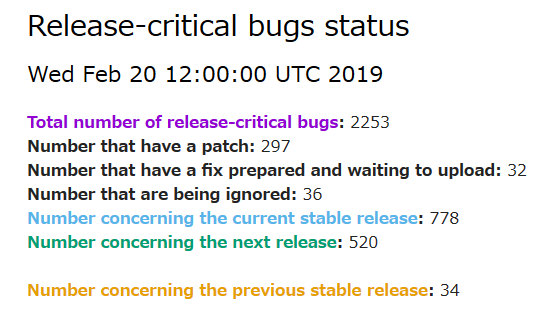
\includegraphics[width=0.5\hsize]{image201902/debian-rcbug-1_20190220.png}
  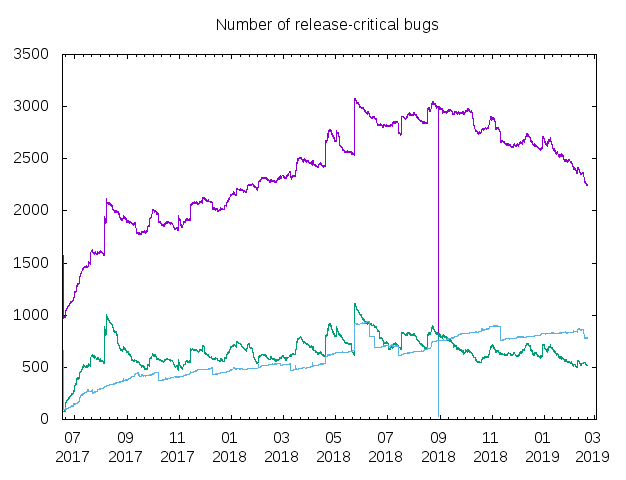
\includegraphics[width=0.5\hsize]{image201902/debian-rcbug-2_20190220.png}
  % https://bugs.debian.org/release-critical/
\end{center}

\end{frame}


\subsection{変更点}

\begin{frame}
  \begin{center}\Huge{変更点}\end{center}
\end{frame}


\begin{frame}{Debian 9 から 10 の変更点}% [containsverbatim]

【ご注意ください】

まだリリースノートは出ていません。今後変わることがあります。

\end{frame}



\begin{frame}{Debian 9 から 10 の変更点}% [containsverbatim]

usr-merge の適用は Buster では見送り

\begin{itemize}
\item \url{https://wiki.debian.org/UsrMerge}
\item /bin,/sbin,/libを、/usr/bin,/usr/sbin,/usr/lib へのシンボリックにすること
\item 一部のパッケージで問題が出たため、技術委員会も含めてBuster ではどうするか 議論になった
  \begin{itemize}
  \item 議論の結果、usr-merge の取り組みは Buster のリリース後に改めて進めことになった
  \item 「tech-ctte: Should debootstrap disable merged /usr by default?」 \url{https://bugs.debian.org/cgi-bin/bugreport.cgi?bug=914897}
  \item 「usrmerge -- plan B?」のスレッドを参照 \url{https://lists.debian.org/debian-devel/2018/11/msg00354.html}
  \end{itemize}
\end{itemize}

\end{frame}


%\begin{frame}{Debian 9 から 10 の変更点}% [containsverbatim]
%
%secure boot
%  
%\begin{itemize}
%\item secure boot対応で問題となるバグはすべて解決済み
%\item 皆さんがお持ちのPCで試した動作結果の報告を募集しています
%  \begin{itemize}
%  \item \url{https://wiki.debian.org/SecureBoot/Testing}
%  \end{itemize}
%\end{itemize}
%    
%\end{frame}


\begin{frame}{Debian 9 から 10 の変更点}% [containsverbatim]

linux kernelとglibcのバージョンアップに伴う変更
  
\begin{itemize}
\item apparmorはデフォルトで有効になる
\item Busterをコンテナ環境で動かす場合の制限
  \begin{itemize}
  \item glibc-2.26以降を採用しており、linux-3.2以降が必要
  \item ホスト側がとても古いサーバの場合に Buster がコンテナ環境で動かない場合あり
  \end{itemize}
\item Busterをホスト環境で動かす場合の制限
  \begin{itemize}
  \item amd64において、古い'virtual syscall' がデフォルトで無効
  \item glibc-2.13以下のシステムはコンテナ環境で動かない
    \begin{itemize}
    \item Debian-7以下、RHEL/CentOS-6 以下が該当
    \end{itemize}
  \item 有効にする場合はカーネルパラメータに vsyscall=emulate を追加
  \end{itemize}
\end{itemize}

\end{frame}


\begin{frame}{Debian 9 から 10 の変更点}% [containsverbatim]

GNOME は Wayland での動作がデフォルト

\begin{itemize}
\item 「GNOME on Xorg」も選べます
\item 他のデスクトップ環境は Xorg で動作します
\item GNOME で Wayland を使う場合に日本語を入力できないことがある
  \begin{itemize}
  \item 日本語入力処理(Input Method)周りに問題が残っており、修正対応中
  \end{itemize}
\end{itemize}

\begin{center}
  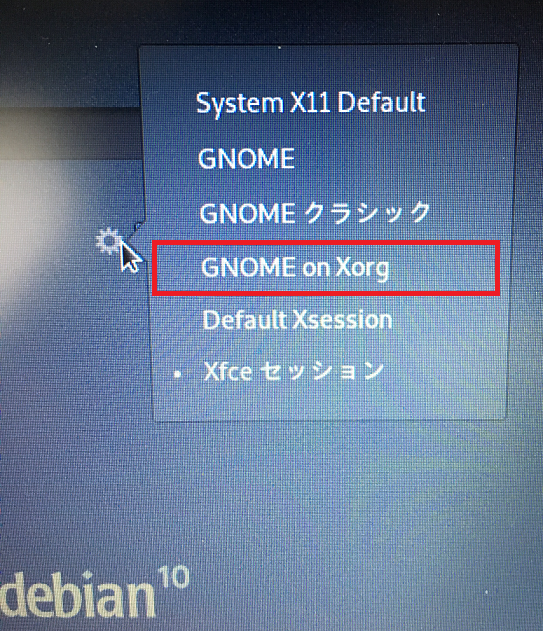
\includegraphics[width=0.5\hsize]{image201902/GDM_GNOME_select_mark.png}
\end{center}

\end{frame}


\begin{frame}{Debian 9 から 10 の変更点}% [containsverbatim]

  \begin{itemize}
  \item openssl-1.1.1系の採用によりTLSv1.3が利用可能
  \item opensshにおいてSSH 1プロトコルが完全削除。SSH 2プロトコルを利用すること。
  \item サポートアーキテクチャはまだ確定していない
    \begin{itemize}
    \item 参考:Debian 9でサポートしているアーキテクチャ
    \item amd64, i386(i686以降), armel, armhf, arm64, mips, mipsel, mips64el, ppc64el, s390x
    \end{itemize}
  \end{itemize}

\end{frame}


\subsection{バグレポート}

\begin{frame}{バグレポートをお願いします}% [containsverbatim]
  \begin{itemize}
  \item 何かおかしい動作や不具合を見つけた場合はバグレポートをお願いします
  \item バグレポートの仕方(レポートは英語で送る必要あり)
    \begin{itemize}
    \item \url{https://www.debian.org/Bugs/Reporting.ja.html}
    \end{itemize}
  \item バグレポートの前にちょっと相談してみたい方は、日本語のDebian JPメーリングリストや、SNSで相談してみてください
    \begin{itemize}
    \item \url{https://www.debian.or.jp/community/ml/openml.html}
    \item Twitter: @debian\_jp
    \end{itemize}
  \end{itemize}
\end{frame}

%-----------------------

\section{Debian Updates}

% 半年間の以下MLから抜粋して紹介する
%  debian-announce@lists.debian.org
%  debian-devel-announce@lists.debian.org

\begin{frame}
  \begin{center}\Huge{Debian Updates}\end{center}
\end{frame}


\subsection{released timeline}

\begin{frame}{Debian Updates}% [containsverbatim]

\begin{itemize}
  \item 2018/11/10:  Updated Debian 9.6  released
  \item 2019/01/23:  Updated Debian 9.7  released
  \item 2019/02/16:  Updated Debian 9.8  released
\end{itemize}

\end{frame}


\subsection{Bits from the DPL}

\begin{frame}{Debian Updates}% [containsverbatim]

Bits from the DPL

\begin{itemize}
\item 月に1回"debian-devel-announce@lists.debian.org"のMLにChrisさんがプロジェクトの進捗を報告している
\item 時間のない方でもこれを読んでおけばDebian Projectの大まかな動きがわかる
\end{itemize}

\small{
\begin{itemize}

\item 2018/10/31 \url{https://lists.debian.org/debian-devel-announce/2018/10/msg00005.html}
\item 2018/11/30 \url{https://lists.debian.org/debian-devel-announce/2018/11/msg00007.html}
\item 2018/12/31 \url{https://lists.debian.org/debian-devel-announce/2018/12/msg00006.html}
\item 2019/01/31 \url{https://lists.debian.org/debian-devel-announce/2019/01/msg00010.html}

\end{itemize}
}

\end{frame}


\subsection{Rust}

\begin{frame}{Debian Updates}% [containsverbatim]

\begin{itemize}
\item 2018/11/02: Rust now available on 14 Debian architectures \\
\ \\
  \small{Rustコンパイラのブートストラップがmips、mips64el、mipsel、powerpcspeでもできるようになった。\url{https://lists.debian.org/debian-devel-announce/2018/11/msg00000.html}}

\end{itemize}

\end{frame}


\subsection{SSH restriction}

\begin{frame}{Debian Updates}% [containsverbatim]

\begin{itemize}
\item 2018/11/10: incoming SSH restriction for *.debian.org \\
\ \\
  \small{debian.orgのドメインを持つ一部のホストにおいて、セキュリティの観点からdebian.orgのサーバからのみssh接続を受け付けるように設定を変更した。\url{https://lists.debian.org/debian-devel-announce/2018/11/msg00003.html}}

\end{itemize}

\end{frame}


\subsection{CTTE vendor-specific patch}

\begin{frame}{Debian Updates}% [containsverbatim]

\begin{itemize}
\item 2018/11/13: CTTE decision on vendor-specific patch series (bug \#904302) \\
\ \\
  \small{DPKGにあるベンダー固有パッチ機能(主に派生ディストリビューションのUbuntuなどが利用している)を継続利用するか利用を止めるか議論があった。議論の結果、Debian 10 Busterのリリース後は利用を止めるべきとの提案がされた。\url{https://lists.debian.org/debian-devel-announce/2018/11/msg00004.html}}

\end{itemize}

\end{frame}


\subsection{GSoC2019}

\begin{frame}{Debian Updates}% [containsverbatim]

\begin{itemize}
\item 2019/01/16: Google Summer of Code 2019\\
\ \\
\small{Google Summer of Code 2019で取り組むプロジェクトのwikiページが立ち上がった。応募の例は、プロジェクトの例は「Android SDK Tools in Debian」、「Continuous Integration for biological applications inside Debian」、「Debian PHP Packaging」、「New Contributor Wizard」「Reproducible Builds」など。\url{https://lists.debian.org/debian-devel-announce/2019/01/msg00007.html}}

\end{itemize}

\end{frame}


%-----------------------

\section{日本語によるDebianの情報}

\begin{frame}\begin{center}\Huge{日本語によるDebianの情報}\end{center}\end{frame}

\begin{frame}{日本語によるDebianの情報}
\begin{itemize}
  \item Debian JP Project \\
      \url{https://www.debian.or.jp}
  \item 東京エリアDebian勉強会\\
      \url{https://tokyodebian-team.pages.debian.net/}
  \item 関西Debian勉強会 \\
      \url{https://wiki.debian.org/KansaiDebianMeeting}
  \item Twitter \\
      \url{@debian_jp}
  \item  雑誌 Software Design 技術評論社発行 \\
    「Debian Hot Topics」、GPG関連の記事など(隔月連載)
\end{itemize}
\end{frame}

%----------------

\section{今後のイベント}

\begin{frame}\begin{center}\Huge{今後のイベント}\end{center}\end{frame}


\begin{frame}{今後のイベント}

\begin{itemize}
\item 2/24(日) 第143関西Debian勉強会
 \begin{itemize}
  \item \url{https://wiki.debian.org/KansaiDebianMeeting/20190224}
  \end{itemize}
\item 3/16(土) 第172回東京エリアDebian勉強会
  \begin{itemize}
  \item \url{https://tokyodebian-team.pages.debian.net/2019-03.html}
  \item セミナー内容は検討中
  \end{itemize}
\end{itemize}

\end{frame}

\end{document}

;;; Local Variables: ***
;;; outline-regexp: "\\([ 	]*\\\\\\(documentstyle\\|documentclass\\|emtext\\|section\\|begin{frame}\\)\\*?[ 	]*[[{]\\|[]+\\)" ***
;;; End: ***
